\section{Partitionnement du serveur}
Un serveur de jeu vidéo classique ne peut gérer qu'un nombre fini de clients. Cependant, les MMOG d'aujourd'hui dépassent largement ce nombre et doivent donc utiliser des méthodes permettant le passage à l'échelle. Pour ce faire, ils partitionnent le serveur de jeu pour lui permettre d'être exécuté sur plusieurs machines.\\

Dans cette partie, nous allons présenter les différentes stratégies de partitionnement utilisées dans les serveurs de jeux vidéos actuels. Ces solutions peuvent être combinées, toutes les combinaisons sont possibles, y compris toutes les solutions en même temps.

\begin{figure}[b!]
	\centering
	\begin{sideways}\qquad\quad~Nombre de joueur\end{sideways}
	\begin{subfigure}[b]{0.5\textwidth}
		\centering
		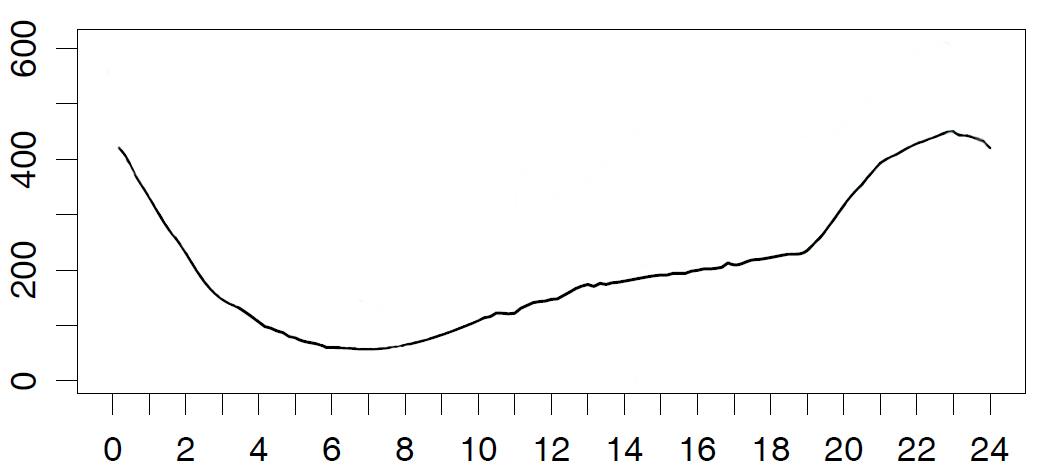
\includegraphics[width=\textwidth]{player_day_evol.png}\\
		Heure
	\end{subfigure}
	\\[0.2cm]
	\caption{Evolution du nombre moyen de joueurs au cours d'une journée sur un royaume de World of Warcraft entre Janvier et Septembre 2006 (voir~\cite{is_server_consolidation_benefical})}
	\label{fig:player_day_evol}
\end{figure}

\subsection{Mouvements des joueurs}
Une des difficultés du partitionnement d'un serveur de MMOG est que la population de ces jeux évolue au cours du temps, à la fois en nombre et en répartition.\\

Comme indiqué dans la \textsc{Figure}~\ref{fig:player_day_evol}, le nombre de joueurs connectés à un serveur jeu varie grandement au cours du temps~\cite{is_server_consolidation_benefical}. En effet, dans une même journée, la période de haute affluence se situe aux alentours de 23h et celle de basse affluence aux alentours de 7h du matin. Ceci s'explique par le fait que les joueurs se connectent en rentrant du travail après le repas et se reposent la nuit. On peut également remarquer que le nombre de joueurs varie aussi au cours de la semaine. Les samedis et dimanches, on observe en moyenne plus de joueurs en globalité (mais un pic maximal identique). Cette variation de joueurs peut entraîner le crash d'un serveur de jeu. On peut observer ce phénomène le premier jour d'un jeu attendu, l'architecture étant totalement saturée par les personnes se connectant à l'heure de sortie du jeu.\\

Il est facile de comprendre dans le cas d'un jeu vidéo qu'il y ait des zones du jeu plus prisées que d'autres. En effet, il existe souvent un but au jeu et les objectifs attirent donc naturellement plus de monde. Dans un MMORPG, les zones correspondant aux villes (qui sont généralement les zones de sociabilisation) et les zones correspondant aux objets les plus rares et puissants sont considérées comme des ``hotspots'' (points chauds) qui correspondent à des centres d'attraction de joueurs. La majeure partie du temps le reste du monde en dehors de ces hotspots reste plutôt vide. Un exemple de ce type de répartition est donné en \textsc{Figure}~\ref{fig:partitionnement_mono}.\\

Ces paramètres variant beaucoup au cours du temps, il faut que le partitionnement puisse s'adapter à ces changements pour être efficace.

\subsection{Séparation des services}
Le but de ce type de partitionnement est de séparer les entités distinctes de l'architecture d'un serveur de jeu vidéo. Les entités usuelles d'un serveur sont:\\

\begin{itemize}
	\item La couche de persistance (usuellement une base de données) qui permet de stocker l'état du jeu.
	\item La couche d'authentification qui permet aux joueurs de se connecter avec leurs identifiants.
	\item La couche logique de jeu qui constitue le traitement des déplacement des éléments du jeu.
	\item La couche service permettant aux administrateurs système d'observer les serveurs (statistiques).\\
\end{itemize}

Cette liste n'est pas exhaustive et n'est pas non plus une liste d'éléments obligatoirement présents sur un serveur de jeu. Cette séparation permet d'éviter d'exécuter toutes les applications sur une même machine et donc qu'une application ne surcharge le processeur et ni n'en pénalise une autre. Elle permet également de mettre en place des techniques de duplication (mirroring) de la base de données pour gérer plus de lectures parallèles. Cela est typiquement utilisé conjointement à un autre partitionnement, par exemple une séparation par zone (voir partie suivante), en utilisant un réplicat par zone.

\begin{figure}[b!]
	\setlength{\fboxsep}{0pt}
		\centering
		\begin{subfigure}[t]{0.22\textwidth}
		\vspace{0pt}
			\framebox{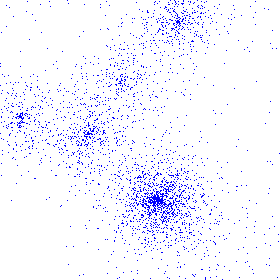
\includegraphics[width=\textwidth]{nuage_mono.png}}
			\caption{Exemple de répartition de la population}
			\label{fig:partitionnement_mono}
		\end{subfigure}
		~
		\begin{subfigure}[t]{0.22\textwidth}
		\vspace{0pt}
			\framebox{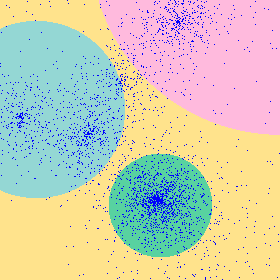
\includegraphics[width=\textwidth]{nuage_zonage.png}}
			\caption{Zoning}
			\label{fig:partitionnement_zonage}
		\end{subfigure}
		~
		\begin{subfigure}[t]{0.22\textwidth}
		\centering
		\vspace{0.5cm}
			\begin{tabular}{*{2}{>{\centering\arraybackslash}m{0.4\textwidth}}}
				\multicolumn{2}{c}{\framebox{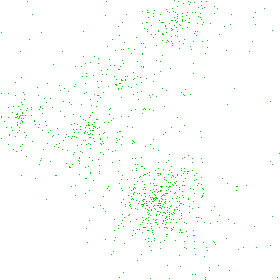
\includegraphics[width=0.4\textwidth]{nuage_sharding_vert.png}}}\\
				\framebox{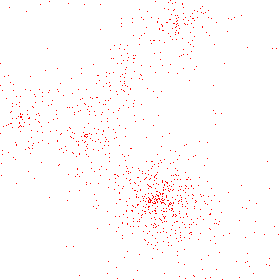
\includegraphics[width=0.4\textwidth]{nuage_sharding_rouge.png}}&
				\framebox{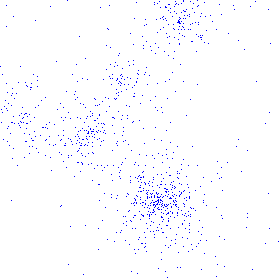
\includegraphics[width=0.4\textwidth]{nuage_sharding_bleu.png}}
			\end{tabular}
		\caption{Sharding}
		\label{fig:partitionnement_sharding}
		\end{subfigure}
		~
		\begin{subfigure}[t]{0.22\textwidth}
		\vspace{0pt}
			\framebox{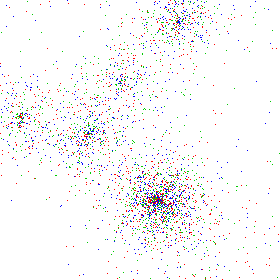
\includegraphics[width=\textwidth]{nuage_cloning.png}}
			\caption{Clonage}
			\label{fig:partitionnement_clonage}
		\end{subfigure}
		\\[0.2cm]
	\caption{Types de partitionnement}
	\label{fig:partitionnement}
\end{figure}

\subsection{Zoning}
Le zoning correspond au découpage du monde du jeu en différentes zones qui peuvent être gérées par des machines différentes, une machine étant donc responsable d'une ou plusieurs zones (voir \textsc{Figure}~\ref{fig:partitionnement_zonage}). Ces zones sont souvent séparées par des limites géographiques dans le monde du jeu (montagnes, rivières, mers...) et sont donc souvent fixes. Les zones ne sont généralement pas transparentes pour les joueurs, ce qui réduit l'immersion dans le jeu car elles sont accompagnées de zone de chargement dans le jeu et l'interaction de deux joueurs à la frontière n'est pas possible.\\

Pour contrer le problème des interactions aux frontières, des techniques de synchronisations inter-serveur peuvent être mises en places pour avoir l'illusion d'un monde sans frontière. Cette solution apporte cependant un coût et une complexité plus élevés. Une méthode pour gérer ce problème est la création de zone de chevauchement (overlap) dont les objets sont gérés par les deux machines en même temps.\\

Les zones étant fixes, un grand nombre de joueurs peut se retrouver dans une même zone et entraîner une surcharge de la machine responsable de cette zone. Pour contrer ceci, on peut partitionner le monde en micro-zones et répartir celles-ci dynamiquement entre les machines du serveur~\cite{triangle_based_load_balancing}. Les micro-zones peuvent également être dynamiques pour être sûr de ne pas en surcharger une. Ceci complexifie les interactions aux frontières car l'architecture est fortement dynamique. Cette solution vient avec un coût de transfert qui peut totalement contrebalancer les bénéfices de cette méthode, voire pénaliser son utilisation, surtout si les zones sont très petites et les transferts nombreux.\\

Cette dernière méthode de partitionnement fonctionne bien mais est complexe. Le zoning est le partitionnement principal de l'architecture que nous allons proposer en partie IV car celui-ci ne sépare pas les joueurs en groupes ne pouvant pas interagir. Ce domaine reste encore un sujet ouvert de la recherche car il est nécessaire de trouver de bons algorithmes permettant le dynamisme des zones.

\subsection{Sharding}
Plutôt que de séparer le monde du jeu en plusieurs zones, cette technique consiste à dupliquer le monde du jeu et à répartir la masse de joueurs en plusieurs groupes qui seront hébergés sur différentes machines ayant chacun une copie du monde du jeu (voir \textsc{Figure}~\ref{fig:partitionnement_sharding}). La majeure partie des MMOG utilisent cette technique en nommant ces groupes shards, royaumes (realm) ou mondes (world). Chaque monde est indépendant et ne peut communiquer. La charge des serveurs est limitée en diminuant le nombre maximum de joueurs par monde. Il suffit ensuite d'ajouter ou de retirer des mondes selon le nombre de joueurs, telles des tables de poker dans un casino. Cependant, tout comme les tables de poker, les joueurs ne jouent pas réellement ensemble.\\

Cette approche sépare les joueurs et limite donc les interactions inter-joueurs à ceux se situant dans le même monde, cette séparation étant souvent fixe. Dans World of Warcraft par exemple, avant la création d'un avatar, il faut choisir le royaume dans lequel on souhaite jouer. Cependant, des options de migrations sont actuellement disponibles dans World of Warcraft pour passer d'un royaume à un autre, coûtant 20\euro{} pour une migration vers n'importe quel serveur et gratuite pour passer d'un serveur à population élevé vers un serveur à population faible. Le prix ne sert pas ici à faire des bénéfices mais à équilibrer la charge entre les serveurs.

\subsection{Instancing}
Cette solution se situe à mi-chemin entre les deux solutions précédentes. Une instance est une copie d'une zone et il peut exister plusieurs copies d'une zone. Un joueur peut interagir avec les autres joueurs de cette instance mais pas avec les joueurs d'une autre instance de cette même zone. Chaque instance hébergeant un nombre limité de joueurs, la charge générée par une unique instance n'est pas grande et plusieurs instances peuvent être attribuées à une seule machine. Elles peuvent également être distribuées dynamiquement entre les machines.\\

Certains joueurs peuvent donc se donner rendez-vous et se retrouver au même endroit sans se voir, ce qui réduit l'immersion du joueur. Dans la plupart des jeux, seules des zones réduites sont instanciées. Celles-ci se font en groupes de joueurs s'étant organisés avant de pénétrer dans la zone instanciée. Ces zones sont la plupart du temps ce qui est appelé ``donjon'' dans les jeux de rôles (endroits fermé). Cela permet à chaque groupe de joueurs d'expérimenter le même contenu au même moment sans subir les interférences d'un autre groupe et cette séparation, bien que nuisant à l'immersion, est donc nécessaire pour des questions de jouabilité.\\

Certains jeux instancient les zones d'affluence telles que les villes et capitales. Cependant, il est dans ce cas souvent possible de changer d'instance à la volée à la demande du joueur pour rejoindre un camarade de jeu par exemple.

\subsection{Autres techniques}
D'autres techniques utilisées sont plus rarement observées.
\paragraph{Clonage\\}
Cette technique répartit le coût du calcul des actions des joueurs sur plusieurs machines gérant conjointement la même zone. Dans certains jeux comme les jeux de stratégie en temps réel (RTS), des calculs sont à effectuer lors d'un clic de déplacement d'un joueur, comme calculer le chemin que vont prendre les unités (pathfinding) ou le déplacement en formation des unités. Ces calculs étant plus lourds, chaque machine est en charge d'un ou plusieurs joueurs et effectue les calculs en parallèle (voir \textsc{Figure}~\ref{fig:partitionnement_clonage}). En cas d'interaction entre deux joueurs n'étant pas gérés par la même machine, il faut mettre en place des mécanismes de verrou de modification pour éviter d'arriver à des résultats incohérents.
\paragraph{Ralentissement du temps\\}
Cette technique consiste à ralentir le déroulement du temps sur le serveur pour permettre au serveur de traiter toutes les actions et de les transmettre aux joueurs. Ainsi le temps entre deux mises à jour pour le client est ralenti. Cette solution est utilisée dans le jeu Eve Online pour les combats de vaisseaux de grande ampleur où la gestion des collisions entre vaisseaux et missiles ainsi que les mouvement des joueurs devient très intensive pour une même zone. Il faut bien sûr remarquer que ce type de solution n'est pas envisageable dans n'importe quel type de jeu car les mécaniques du jeu ne s'y prêtent pas forcément. Par exemple, un jeu de tir à la première personne (FPS), basé sur les réflexes, nécessite des actions rapides. Dans ce cas, ce genre de solution n'est pas utilisable.

\subsection{Conclusion}
La mise en place de ces techniques de partitionnement par les développeurs de MMOG montre qu'il existe un réel problème de passage à l'échelle. Dans la majorité des cas, l'ensemble des joueurs est séparé en plus petits groupes pour limiter le nombre de joueurs en interaction. Cela permet de ramener le nombre de joueurs à un nombre pouvant être géré par les architectures existantes décrites en partie III. Ceci montre qu'il y a donc un besoin en solutions permettant à tous les joueurs de jouer réellement ensemble.
